\documentclass{ximera}
\usepackage{OERLinearAlgebra}


\usepackage{mathtools}
\usepackage{tikz-3dplot}
\newcommand\norm[1]{\left\lVert#1\right\rVert}

\author{Anna Davis \and Rosemarie Emanuele} \title{Vector Arithmetic} \license{CC-BY 4.0}

\begin{document}

\begin{abstract}
 We define vector addition and scalar multiplication algebraically and geometrically.
\end{abstract}
\maketitle



\section*{Geometry of Scalar Multiplication} The product of vector $\vec{u}$ with a positive scalar $k$, is a vector $k\vec{u}$ that points in the same direction as $\vec{u}$, and whose length  is equal to the length of $\vec{u}$ multiplied by $k$. For example, the figure below shows vectors $\vec{u}$ and $2\vec{u}$.  The vectors point in the same direction but the magnitude of $2\vec{u}$ is twice the magnitude of $\vec{u}$.

\begin{image}[1.5in]
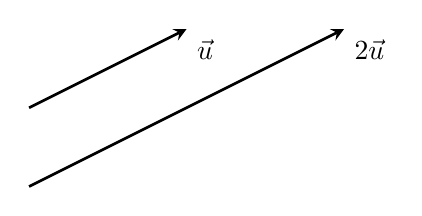
\begin{tikzpicture}
\draw[line width=1pt,-stealth](-1,0)--(1,1)node[below right]{$\vec{u}$};
\draw[line width=1pt,-stealth](-1,-1)--(3,1)node[below right]{$2\vec{u}$};
 \end{tikzpicture}
\end{image}


If a vector $\vec{u}$ is multiplied by $-1$, the resulting vector is denoted by $-\vec{u}$.  It has the same length as vector $\vec{u}$, but points in the opposite direction.

\begin{image}[0.8in]
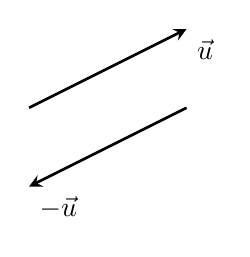
\begin{tikzpicture}
\draw[line width=1pt,-stealth](-1,0)--(1,1)node[below right]{$\vec{u}$};
\draw[line width=1pt,-stealth](1,0)--(-1,-1)node[below right]{$-\vec{u}$};
 \end{tikzpicture}
\end{image}



\section*{Algebra of Scalar Multiplication}
We know what scalar multiplication accomplishes geometrically.  Our goal now is to translate this idea to an algebraic operation.  

\begin{initprob}\label{init:scalarmult} Consider vector $\vec{u}=\begin{bmatrix}4\\2\end{bmatrix}$.  We will find an algebraic approach for multiplying $\vec{u}$ by $\frac{1}{2}$. 

\begin{image}[2.5in]
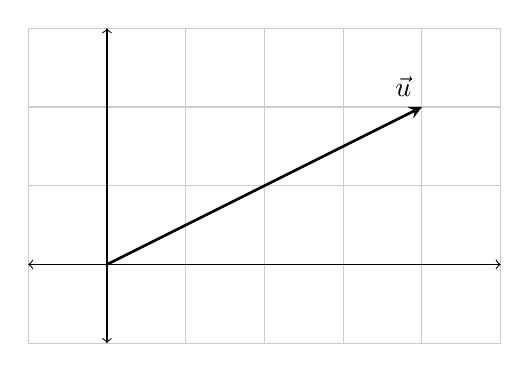
\begin{tikzpicture}[scale=1]
\draw[thin,gray!40] (-1,-1) grid (5,3);
  \draw[<->] (-1,0)--(5,0);
  \draw[<->] (0,-1)--(0,3);
  
 \draw[line width=1pt,-stealth](0,0)--(4,2)node[above left]{$\vec{u}$};
%  \draw[line width=2pt,red,-stealth](0,0)--(2,1) node[above left]{$[2,1]$};
 \end{tikzpicture}
\end{image}

Consider $\vec{u}$ to be the hypotenuse of a right triangle.  

\begin{image}[2.5in]
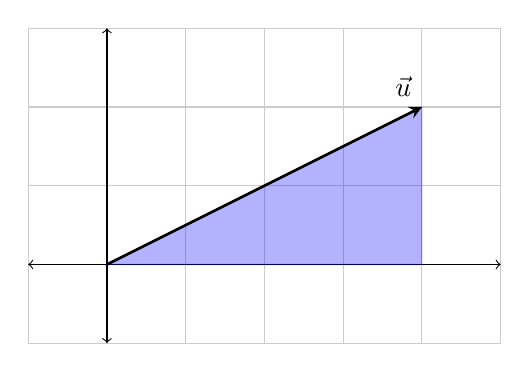
\begin{tikzpicture}[scale=1]
\draw[thin,gray!40] (-1,-1) grid (5,3);
  \draw[<->] (-1,0)--(5,0);
  \draw[<->] (0,-1)--(0,3);
   \filldraw[blue, opacity=0.3](0,0)--(4,2)--(4,0)--cycle;
 \draw[line width=1pt,-stealth](0,0)--(4,2)node[above left]{$\vec{u}$};
%  \draw[line width=2pt,red,-stealth](0,0)--(2,1) node[above left]{$[2,1]$};
 \end{tikzpicture}
\end{image}

The head of $\frac{1}{2}\vec{u}$ should be the midpoint of the hypotenuse.

\begin{image}[2.5in]
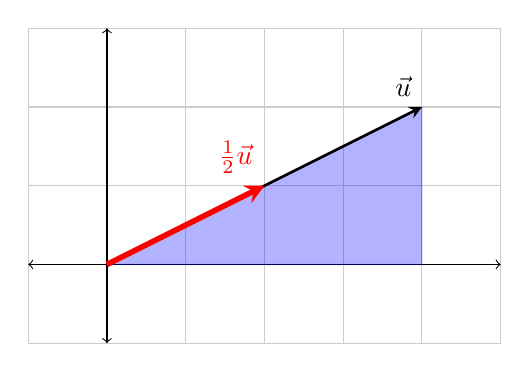
\begin{tikzpicture}[scale=1]
\draw[thin,gray!40] (-1,-1) grid (5,3);
  \draw[<->] (-1,0)--(5,0);
  \draw[<->] (0,-1)--(0,3);
   \filldraw[blue, opacity=0.3](0,0)--(4,2)--(4,0)--cycle;
 \draw[line width=1pt,-stealth](0,0)--(4,2)node[above left]{$\vec{u}$};
 \draw[line width=2pt,red,-stealth](0,0)--(2,1) node[above left]{$\frac{1}{2}\vec{u}$};
 \end{tikzpicture}
\end{image}

From geometry we know that if we drop perpendiculars from the midpoint of the hypotenuse to the two legs of the triangle, the perpendiculars will bisect the legs.

\begin{image}[2.5in]
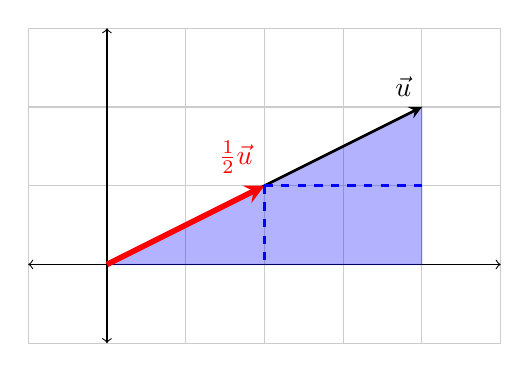
\begin{tikzpicture}[scale=1]
\draw[thin,gray!40] (-1,-1) grid (5,3);
  \draw[<->] (-1,0)--(5,0);
  \draw[<->] (0,-1)--(0,3);
   \filldraw[blue, opacity=0.3](0,0)--(4,2)--(4,0)--cycle;
 \draw[line width=1pt,-stealth](0,0)--(4,2)node[above left]{$\vec{u}$};
 \draw[line width=2pt,red,-stealth](0,0)--(2,1) node[above left]{$\frac{1}{2}\vec{u}$};
  \draw[line width=1pt,blue, dashed](2,1)--(2,0);
   \draw[line width=1pt,blue, dashed](2,1)--(4,1);
 \end{tikzpicture}
\end{image}
This tells us that to find $x$ and $y$ components of $\frac{1}{2}\vec{u}$ we must multiply each component of $\vec{u}$ by $\frac{1}{2}$.
$$\frac{1}{2}\vec{u}=(1/2)\begin{bmatrix}4\\2\end{bmatrix}=\begin{bmatrix}(1/2)(4)\\(1/2)(2)\end{bmatrix}=\begin{bmatrix}2\\1\end{bmatrix}$$
\end{initprob}

\begin{initprob}\label{init:negscalarmult} Consider vector $\vec{v}=\begin{bmatrix}3\\1\end{bmatrix}$
It is clear that multiplying the components of $\vec{v}$ by $-1$ reverses the direction of $\vec{v}$ while preserving its magnitude.

\begin{image}[3in]
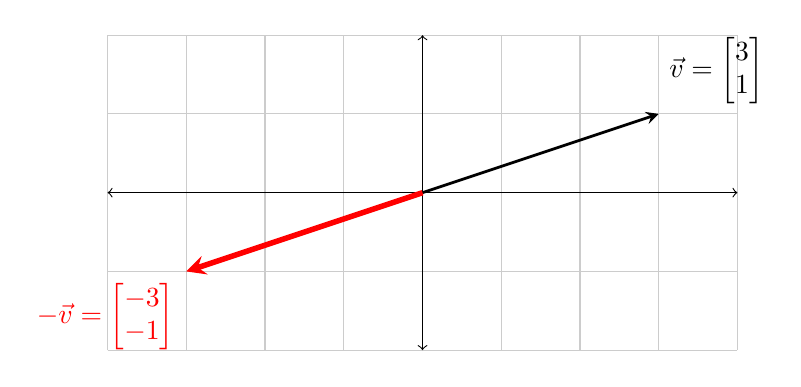
\begin{tikzpicture}[scale=1]
\draw[thin,gray!40] (-4,-2) grid (4,2);
  \draw[<->] (-4,0)--(4,0);
  \draw[<->] (0,-2)--(0,2);
  
 \draw[line width=1pt,-stealth](0,0)--(3,1)node[above right]{$\vec{v}=\begin{bmatrix}3\\1\end{bmatrix}$};
  \draw[line width=2pt,red,-stealth](0,0)--(-3,-1) node[below left]{$-\vec{v}=\begin{bmatrix}-3\\-1\end{bmatrix}$};
 \end{tikzpicture}
\end{image}

\end{initprob}

Exploration Problems  \ref{init:scalarmult} and \ref{init:negscalarmult} give rise to the following definition of scalar multiplication.


  \begin{definition} 
  
Let $\vec{u}=\begin{bmatrix}
u_1\\
u_2\\
\vdots\\
u_n
\end{bmatrix}$ be a vector in $\RR^n$, and let $k$ be a scalar, then
  $$k\vec{u}=k\begin{bmatrix}
u_1\\
u_2\\
\vdots\\
u_n
\end{bmatrix}=\begin{bmatrix}
ku_1\\
ku_2\\
\vdots\\
ku_n
\end{bmatrix}$$
  \end{definition}
If $\vec{v}=k\vec{u}$ ($k\neq 0$), then $\vec{u}=\frac{1}{k}\vec{v}$, and we say that $\vec{v}$ and $\vec{u}$ are \dfn{scalar multiples of each other}.

\section*{Geometry of Vector Addition} 
There are two ways to add vectors geometrically.  
\subsection*{``Head-to-Tail" Addition Method}
Given vectors $\vec{v}$ and $\vec{u}$, we can find the sum $\vec{v}+\vec{u}$ by sliding $\vec{u}$ so as to place its tail at the head of vector $\vec{v}$.  The vector connecting the tail of $\vec{v}$ with the head of $\vec{u}$ is the sum $\vec{v}+\vec{u}$, as shown in the figure below.    
\begin{image}[4in]
\begin{tikzpicture}
\draw[line width=1pt,-stealth,red](-1,-2)--(2,-3)node[below right]{$\vec{u}$};
\draw[line width=1pt,-stealth, blue](-1,-1)--(3,1)node[above right]{$\vec{v}$};
 \end{tikzpicture}
 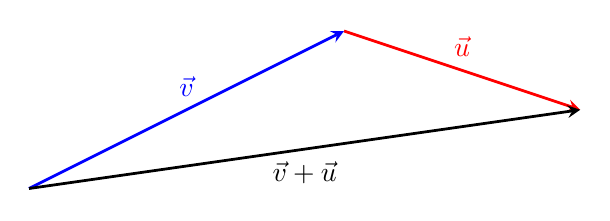
\begin{tikzpicture}
\draw[line width=1pt,-stealth,red](3,3)--(6,2);
\draw[line width=1pt,-stealth, blue](-1,1)--(3,3);
\draw[line width=1pt,-stealth](-1,1)--(6,2);

 \node[blue] at (1, 2.3)   (a) {$\vec{v}$};
 \node[red] at (4.5, 2.8)   (a) {$\vec{u}$};
  \node[black] at (2.5, 1.2)   (a) {$\vec{v}+\vec{u}$};
 \end{tikzpicture}
\end{image}

This sum can be interpreted as the total displacement that occurs when traveling along the two vectors starting at the tail of $\vec{v}$ and finishing at the head of $\vec{u}$.

Note that if we place the tail of $\vec{v}$ at the head of $\vec{u}$ instead, the sum vector $\vec{u}+\vec{v}$ will be the same as $\vec{v}+\vec{u}$.  Thus, addition of vectors is commutative.
\subsection*{Parallelogram Addition Method}
Most of the time we deal with vectors in standard position.  So all vector tails are located at the origin.  This motivates the {\it parallelogram} method for adding vectors.  

Observe that if we slide vectors $\vec{u}$ and $\vec{v}$ so that their tails are together, the two vectors determine a parallelogram.  

\begin{image}[2.5in]
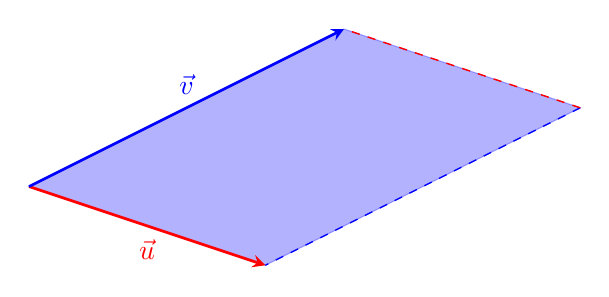
\begin{tikzpicture}
\filldraw[blue, opacity=0.3](-1,1)--(2,0)--(6,2)--(3,3)--cycle;
 \draw[line width=0.5pt,blue,dashed](6,2)--(2,0);
  \draw[line width=0.5pt,red, dashed](6,2)--(3,3);
 
\draw[line width=1pt,-stealth,red](-1,1)--(2,0);
\draw[line width=1pt,-stealth, blue](-1,1)--(3,3);
%\draw[line width=1pt,-stealth](-1,1)--(6,2);

 \node[blue] at (1, 2.3)   (a) {$\vec{v}$};
 \node[red] at (0.5, 0.2)   (a) {$\vec{u}$};
 
  
 \end{tikzpicture}
\end{image}

Opposite sides of a parallelogram are congruent and parallel.

\begin{image}[2.5in]
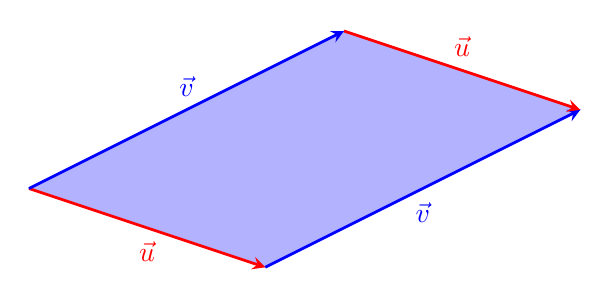
\begin{tikzpicture}
\filldraw[blue, opacity=0.3](-1,1)--(2,0)--(6,2)--(3,3)--cycle;
 \draw[line width=1pt,-stealth, blue](2,0)--(6,2);
  \draw[line width=1pt,red, -stealth](3,3)--(6,2);
 
\draw[line width=1pt,-stealth,red](-1,1)--(2,0);
\draw[line width=1pt,-stealth, blue](-1,1)--(3,3);
%\draw[line width=1pt,-stealth](-1,1)--(6,2);

 \node[blue] at (1, 2.3)   (a) {$\vec{v}$};
 \node[red] at (0.5, 0.2)   (a) {$\vec{u}$};
 
 \node[blue] at (4, 0.7)   (a) {$\vec{v}$};
 \node[red] at (4.5, 2.8)   (a) {$\vec{u}$};
 
  
 \end{tikzpicture}
\end{image}

Applying the ``head-to-tail" addition method shows that the sum $\vec{v}+\vec{u}$ is the diagonal of the parallelogram determined by $\vec{v}$ and $\vec{u}$.

\begin{image}[2.5in]
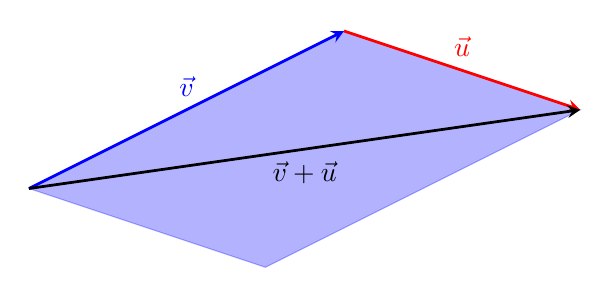
\begin{tikzpicture}
\filldraw[blue, opacity=0.3](-1,1)--(2,0)--(6,2)--(3,3)--cycle;
% \draw[line width=1pt,-stealth, blue](2,0)--(6,2);
  \draw[line width=1pt,red, -stealth](3,3)--(6,2);
 
%\draw[line width=1pt,-stealth,red](-1,1)--(2,0);
\draw[line width=1pt,-stealth, blue](-1,1)--(3,3);
\draw[line width=1pt,-stealth](-1,1)--(6,2);

 \node[blue] at (1, 2.3)   (a) {$\vec{v}$};

 \node[red] at (4.5, 2.8)   (a) {$\vec{u}$};
  \node[black] at (2.5, 1.2)   (a) {$\vec{v}+\vec{u}$};
  
 \end{tikzpicture}
\end{image}

%\begin{image}[4in]
%\begin{tikzpicture}
%\draw[line width=1pt,-stealth,red](-1,-2)--(2,-3)node[below right]{$\vec{u}$};
%\draw[line width=1pt,-stealth, blue](-1,-1)--(3,1)node[above right]{$\vec{v}$};
% \end{tikzpicture}
% \begin{tikzpicture}
% \draw[line width=0.5pt,blue,dashed](6,2)--(2,0);
%  \draw[line width=0.5pt,red, dashed](6,2)--(3,3);
 
%\draw[line width=1pt,-stealth,red](-1,1)--(2,0);
%\draw[line width=1pt,-stealth, blue](-1,1)--(3,3);
%\draw[line width=1pt,-stealth](-1,1)--(6,2);

 %\node[blue] at (1, 2.3)   (a) {$\vec{v}$};
 %\node[red] at (0.5, 0.2)   (a) {$\vec{u}$};
  %\node[black] at (2.5, 1.2)   (a) {$\vec{u}+\vec{v}$};
  
 %\end{tikzpicture}
%\end{image}



\section*{Algebra of Vector Addition}

We now know how to add vectors geometrically.  Our next goal is to translate this idea to an algebraic operation.  

\begin{initprob}\label{init:vectoradd} In this problem we will find the sum of $\vec{u}=\begin{bmatrix}5\\1\end{bmatrix}$ and $\vec{v}=\begin{bmatrix}2\\3\end{bmatrix}$.


\begin{image}[3.5in]
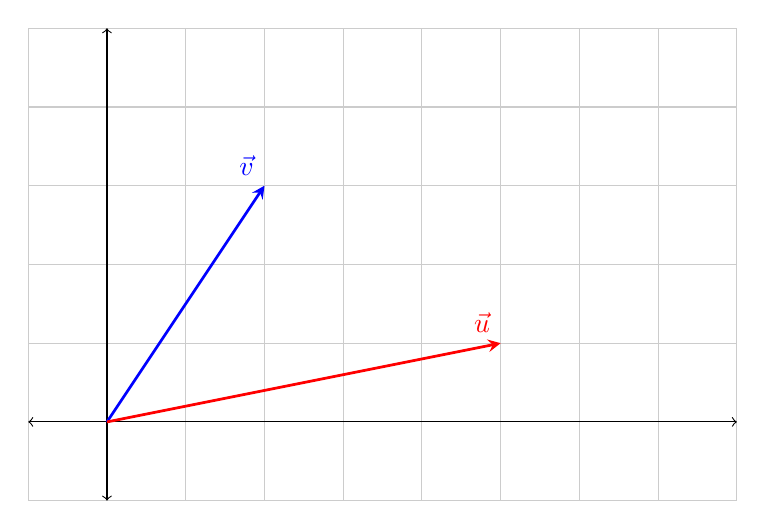
\begin{tikzpicture}[scale=1]
\draw[thin,gray!40] (-1,-1) grid (8,5);
  \draw[<->] (-1,0)--(8,0);
  \draw[<->] (0,-1)--(0,5);
   
 \draw[line width=1pt,blue,-stealth](0,0)--(2,3)node[above left]{$\vec{v}$};
 \draw[line width=1pt,red,-stealth](0,0)--(5,1) node[above left]{$\vec{u}$};

 \end{tikzpicture}
\end{image}

To use ``head-to-tail" addition method, or to construct the side of a parallelogram opposite of $\vec{u}$, we want to slide $\vec{u}$ so that its tail is at the point $(2, 3)$. Observe that $\vec{u}$ has a ``run" of $5$ and a ``rise" of $1$.  If we start at $(2, 3)$, go over $5$ then up $1$, we will land on $(7, 4)$.

\begin{image}[3.5in]
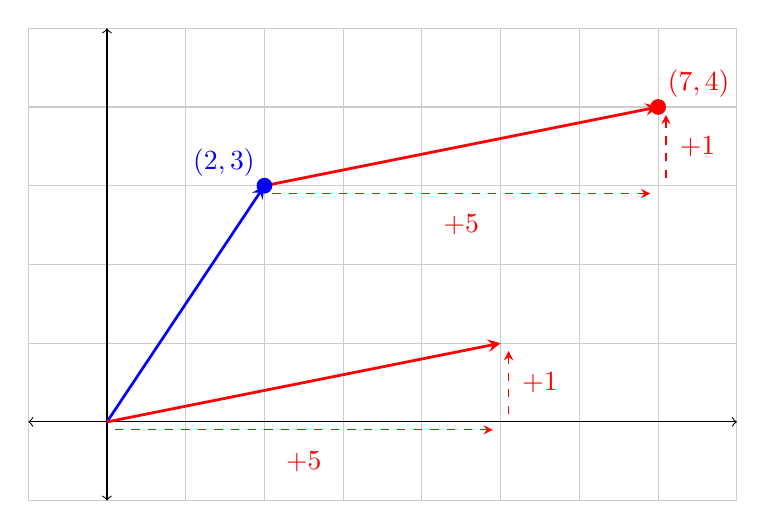
\begin{tikzpicture}[scale=1]
\draw[thin,gray!40] (-1,-1) grid (8,5);
  \draw[<->] (-1,0)--(8,0);
  \draw[<->] (0,-1)--(0,5);
   
 \draw[line width=1pt,blue,-stealth](0,0)--(2,3);
 \draw[line width=1pt,red,-stealth](0,0)--(5,1);
 
\draw[line width=1pt,red,-stealth](2,3)--(7,4);
 
  \draw[line width=0.5pt,red, dashed,-stealth](2.1,2.9)--(6.9,2.9);
   \draw[line width=0.5pt,red, dashed, -stealth](7.1,3.1)--(7.1,3.9);
   
    \draw[line width=0.5pt,red, dashed,-stealth](0.1,-0.1)--(4.9,-0.1);
   \draw[line width=0.5pt,red, dashed, -stealth](5.1,0.1)--(5.1,0.9);
   
   \fill[blue] (2,3)node[above left]{$(2,3)$} circle (0.1cm);
   \fill[red] (7,4)node[above right]{$(7,4)$} circle (0.1cm);
   
   \node[red] at (2.5, -0.5)   (b) {$+5$};
   \node[red] at (4.5, 2.5)   (b) {$+5$};
   \node[red] at (5.5, 0.5)   (b) {$+1$};
   \node[red] at (7.5, 3.5)   (b) {$+1$};
 \end{tikzpicture}
\end{image}

The sum $\vec{u}+\vec{v}$ is shown below.

\begin{image}[3.5in]
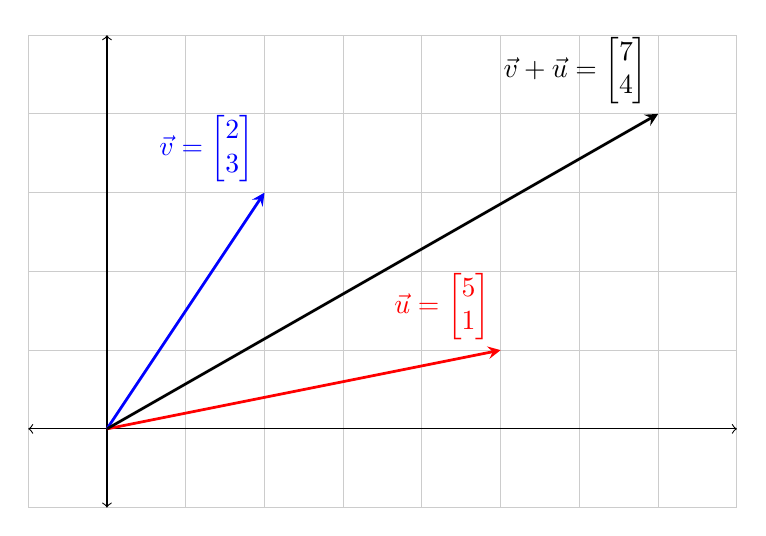
\begin{tikzpicture}[scale=1]
\draw[thin,gray!40] (-1,-1) grid (8,5);
  \draw[<->] (-1,0)--(8,0);
  \draw[<->] (0,-1)--(0,5);
   
 \draw[line width=1pt,blue,-stealth](0,0)--(2,3)node[above left]{$\vec{v}=\begin{bmatrix}2\\3\end{bmatrix}$};
 \draw[line width=1pt,red,-stealth](0,0)--(5,1) node[above left]{$\vec{u}=\begin{bmatrix}5\\1\end{bmatrix}$};
 
\draw[line width=1pt,-stealth](0,0)--(7,4) node[above left]{$\vec{v}+\vec{u}=\begin{bmatrix}7\\4\end{bmatrix}$};

 \end{tikzpicture}
\end{image}
We see that the components of $\vec{v}+\vec{u}$ can be found by adding the components of $\vec{v}$ and $\vec{u}$.
$$\vec{v}+\vec{u}=\begin{bmatrix}2\\3\end{bmatrix}+\begin{bmatrix}5\\1\end{bmatrix}=\begin{bmatrix}7\\4\end{bmatrix}$$
\end{initprob}

Exploration Problem \ref{init:vectoradd} motivates the following definition.
  \begin{definition}\label{def:vectoradd} 
  Let $\vec{u}=\begin{bmatrix}
u_1\\
u_2\\
\vdots\\
u_n
\end{bmatrix}$ and $\vec{v}=\begin{bmatrix}
v_1\\
v_2\\
\vdots\\
v_n
\end{bmatrix}$ be vectors in $\RR^n$.  We define $\vec{u}+\vec{v}$ by
  $$\vec{u}+\vec{v}=\begin{bmatrix}
u_1\\
u_2\\
\vdots\\
u_n
\end{bmatrix}+\begin{bmatrix}
v_1\\
v_2\\
\vdots\\
v_n
\end{bmatrix}=\begin{bmatrix}
u_1+v_1\\
u_2+v_2\\
\vdots\\
u_n+v_n
\end{bmatrix}$$
  
\end{definition}

\section*{Vector Subtraction}
We can find the difference of two vectors by interpreting subtraction as ``addition of the opposite".  Thus,
$$\vec{v}-\vec{u}=\vec{v}+(-\vec{u})$$
Vector subtraction has an interesting geometric interpretation.  As shown in the figure below, if $\vec{v}+\vec{u}$ is a diagonal of the parallelogram determined by $\vec{v}$ and $\vec{u}$, the difference $\vec{v}-\vec{u}$ is the other diagonal of the same parallelogram.

\begin{image}[4.5in]
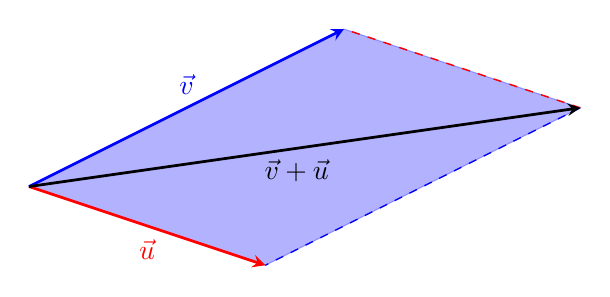
\begin{tikzpicture}
\filldraw[blue, opacity=0.3](-1,1)--(2,0)--(6,2)--(3,3)--cycle;
 \draw[line width=0.5pt,blue,dashed](6,2)--(2,0);
  \draw[line width=0.5pt,red, dashed](6,2)--(3,3);
 
\draw[line width=1pt,-stealth,red](-1,1)--(2,0);
\draw[line width=1pt,-stealth, blue](-1,1)--(3,3);
\draw[line width=1pt,-stealth](-1,1)--(6,2);

 \node[blue] at (1, 2.3)   (a) {$\vec{v}$};
 \node[red] at (0.5, 0.2)   (a) {$\vec{u}$};
 \node[black] at (2.4, 1.2)   (a) {$\vec{v}+\vec{u}$};
 \end{tikzpicture}
 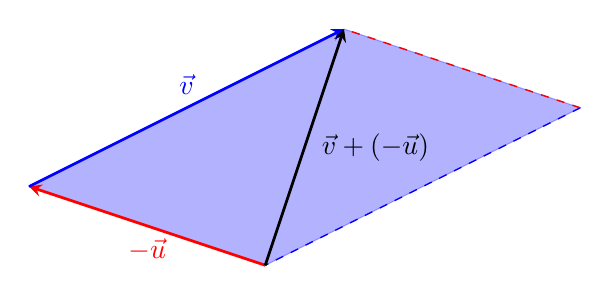
\begin{tikzpicture}
\filldraw[blue, opacity=0.3](-1,1)--(2,0)--(6,2)--(3,3)--cycle;
 \draw[line width=0.5pt,blue,dashed](6,2)--(2,0);
  \draw[line width=0.5pt,red, dashed](6,2)--(3,3);
\draw[line width=1pt,-stealth,red](2,0)--(-1,1); 
\draw[line width=1pt,-stealth, blue](-1,1)--(3,3);
\draw[line width=1pt,-stealth](2,0)--(3,3);

 \node[blue] at (1, 2.3)   (a) {$\vec{v}$};
 \node[red] at (0.5, 0.2)   (a) {$-\vec{u}$};
  \node[black] at (3.4, 1.5)   (a) {$\vec{v}+(-\vec{u})$};
 \end{tikzpicture}
\end{image}
\section*{Properties of Vector Addition and Scalar Multiplication}
  \begin{theorem}\label{th:vecproperties} The following properties hold for vectors $\vec{u}$, $\vec{v}$ and ${\bf w}$ in $\RR^n$ and scalars $k$ and $p$.
  \begin{enumerate}
  \item \label{item:commvectoradd}
  Commutative Property of Addition
  $$\vec{u}+\vec{v}=\vec{v}+\vec{u}$$
  \item \label{item:assocvectoradd}
  Associative Property of Addition
  $$(\vec{u}+\vec{v})+{\bf w}=\vec{u}+(\vec{v}+{\bf w})$$
  \item \label{item:identityvectoradd}
  Existence of Additive Identity
  $$\vec{u}+\vec{0}=\vec{u}$$
  \item \label{item:inversevectoradd}
  Existence of Additive Inverse
  $$\vec{u}+(-\vec{u})=\vec{0}$$
  \item\label{item:distvectoradd}
  Distributive Property over Vector Addition
  $$k(\vec{u}+\vec{v})=k\vec{u}+k\vec{v}$$
  \item\label{item:distvectoradd2}
  Distributive Property over Scalar Addition
  $$(k+p)\vec{u}=k\vec{u}+p\vec{u}$$
  \item \label{item:assocvectorscalarmult}
  Associative Property for Scalar Multiplication
  $$k(p\vec{u})=(kp)\vec{u}$$
  \item \label{item:onevectorscalarmult}
  Multiplication by 1
  $$1\vec{u}=\vec{u}$$
  \end{enumerate}
\end{theorem}

We will prove Property \ref{item:distvectoradd}.  Proofs of the remaining properties are left to the reader.
\begin{proof}[Proof of Property \ref{item:distvectoradd}]
$$
k(\vec{u}+\vec{v})=k\Bigg(\begin{bmatrix}
u_1\\
u_2\\
\vdots\\
u_n
\end{bmatrix}+\begin{bmatrix}
v_1\\
v_2\\
\vdots\\
v_n
\end{bmatrix}\Bigg)=k\begin{bmatrix}
u_1+v_1\\
u_2+v_2\\
\vdots\\
u_n+v_n
\end{bmatrix}=\begin{bmatrix}
k(u_1+v_1)\\
k(u_2+v_2)\\
\vdots\\
k(u_n+v_n)
\end{bmatrix}=$$
$$=\begin{bmatrix}
ku_1+kv_1\\
ku_2+kv_2\\
\vdots\\
ku_n+kv_n
\end{bmatrix}=\begin{bmatrix}
ku_1\\
ku_2\\
\vdots\\
ku_n
\end{bmatrix}+\begin{bmatrix}
kv_1\\
kv_2\\
\vdots\\
kv_n
\end{bmatrix}=k\begin{bmatrix}
u_1\\
u_2\\
\vdots\\
u_n
\end{bmatrix}+k\begin{bmatrix}
v_1\\
v_2\\
\vdots\\
v_n
\end{bmatrix}
=k\vec{u}+k\vec{v}$$
\end{proof}



\section*{Practice Problems}
 
 \begin{problem}
The figure below shows vectors $\vec{u}$ and $\vec{v}$.  Sketch each of the following in the same coordinate plane.
 
\begin{image}[2.5in]
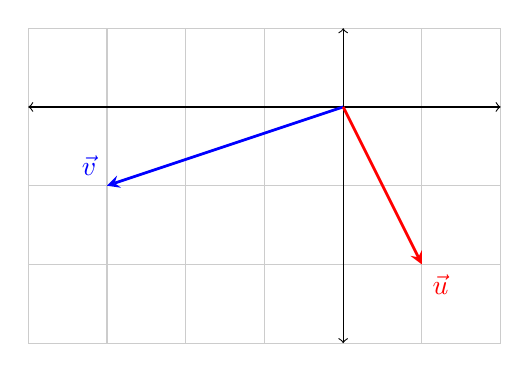
\begin{tikzpicture}[scale=1]
\draw[thin,gray!40] (-4,-3) grid (2,1);
  \draw[<->] (-4,0)--(2,0);
  \draw[<->] (0,-3)--(0,1);
   
 \draw[line width=1pt,blue,-stealth](0,0)--(-3,-1)node[above left]{$\vec{v}$};
 \draw[line width=1pt,red,-stealth](0,0)--(1,-2) node[below right]{$\vec{u}$};

 \end{tikzpicture}
\end{image}
 \begin{enumerate}
  \item 
  $\vec{u}+\vec{v}$
  \item
  $2\vec{u}-\vec{v}$
  \item 
  $3\vec{v}$
  \item
  $-2\vec{u}$
  \end{enumerate}
\end{problem}

\begin{problem} Let $$\vec{u}=\begin{bmatrix}-2\\1\\4\end{bmatrix},\quad\vec{v}\begin{bmatrix}3\\-1\\0\end{bmatrix}$$
Find each of the following
\begin{problem}
$$2\vec{u}-\vec{v}=\begin{bmatrix}\answer{-7}\\\answer{3}\\\answer{8}\end{bmatrix}$$
\end{problem}
\begin{problem} The additive inverse of $\vec{v}$ is
$$\begin{bmatrix}\answer{-3}\\\answer{1}\\\answer{0}\end{bmatrix}$$
\end{problem}
\end{problem}

\begin{problem}
Prove Properties \ref{item:commvectoradd}-\ref{item:inversevectoradd} of Theorem \ref{th:vecproperties}.
\end{problem}

\begin{problem}
Prove Properties \ref{item:distvectoradd2}-\ref{item:onevectorscalarmult} of Theorem \ref{th:vecproperties}.
\end{problem}
 
\end{document} 